%%%%%%%%%%%%%%%%%%%%%%%%%%%%%%%%%%%%%%%%%%%%%%%%%%
% Basic setup. Most papers should leave these options alone.
\documentclass[fleqn,usenatbib]{mnras}

% MNRAS is set in Times font. If you don't have this installed (most LaTeX
% installations will be fine) or prefer the old Computer Modern fonts, comment
% out the following line
\usepackage{newtxtext,newtxmath}
% Depending on your LaTeX fonts installation, you might get better results with one of these:
%\usepackage{mathptmx}
%\usepackage{txfonts}

% Use vector fonts, so it zooms properly in on-screen viewing software
% Don't change these lines unless you know what you are doing
\usepackage[T1]{fontenc}

% Allow "Thomas van Noord" and "Simon de Laguarde" and alike to be sorted by "N" and "L" etc. in the bibliography.
% Write the name in the bibliography as "\VAN{Noord}{Van}{van} Noord, Thomas"
\DeclareRobustCommand{\VAN}[3]{#2}
\let\VANthebibliography\thebibliography
\def\thebibliography{\DeclareRobustCommand{\VAN}[3]{##3}\VANthebibliography}


%%%%% AUTHORS - PLACE YOUR OWN PACKAGES HERE %%%%%

% Only include extra packages if you really need them. Common packages are:
\usepackage{graphicx}	% Including figure files
\usepackage{amsmath}	% Advanced maths commands
\usepackage{amssymb}	% Extra maths symbols

%%%%%%%%%%%%%%%%%%%%%%%%%%%%%%%%%%%%%%%%%%%%%%%%%%

%%%%% AUTHORS - PLACE YOUR OWN COMMANDS HERE %%%%%

% Please keep new commands to a minimum, and use \newcommand not \def to avoid
% overwriting existing commands. Example:
%\newcommand{\pcm}{\,cm$^{-2}$}	% per cm-squared

%%%%%%%%%%%%%%%%%%%%%%%%%%%%%%%%%%%%%%%%%%%%%%%%%%

%%%%%%%%%%%%%%%%%%% TITLE PAGE %%%%%%%%%%%%%%%%%%%

% Title of the paper, and the short title which is used in the headers.
% Keep the title short and informative.
\title[Hot Accretion in FIRE]{Galactic discs fed by hot accretion in the FIRE simulations}

% The list of authors, and the short list which is used in the headers.
% If you need two or more lines of authors, add an extra line using \newauthor
\author[\ldots]{
\ldots,$^{1}$\thanks{E-mail: mn@ras.org.uk (KTS)}
\\
% List of institutions
$^1$ \ldots
}

% These dates will be filled out by the publisher
\date{Accepted XXX. Received YYY; in original form ZZZ}

% Enter the current year, for the copyright statements etc.
\pubyear{2020}

% Don't change these lines

\newcommand{\Rcool}{R_{T=10^5\,{\rm K}}}
\newcommand{\tcon}{t_{T=10^5\,{\rm K}}}
\newcommand{\Mdot}{\dot{M}}
\newcommand{\Rcirc}{R_{\rm circ}} %need better name as R_cool means something else
\newcommand{\Rvir}{R_{\rm vir}}

\begin{document}
\label{firstpage}
\pagerange{\pageref{firstpage}--\pageref{lastpage}}
\maketitle

% Abstract of the paper
\begin{abstract}
We study how gas accretes onto $\sim L^\star$ star-forming galaxies at redshift $z\sim0$ using the FIRE cosmological simulations. We evaluate the relative importance of three different modes of accretion: 
gas that never heats to the virial temperature (``cold accretion''), 
cool clouds which condense out of the hot halo, lose buoyancy and accrete  (``condensation''), 
and inflowing hot gas which remains hot down to the galaxy scale (``cooling flow''). 
We demonstrate that across our sample of $xx$ MW-mass halos most accretion occurs via a cooling flow, accounting for $yy-zz\%$ of all accreted gas. Gas accreted in this mode is hot and quasi-spherical down to $\lesssim 0.1$ of the halo virial radius, at which point it simulataneously cools and circularizes, thus joining the outskirts of the galactic disc. 
% Only a small fraction ($zz$\%) of this hot flow experienced condensation and reheating prior to accretion. 
The remaining $vv-ww\%$ of accreted gas originates in cool clouds which condensed out of the halo. Cold accretion does not occur in appreciable quantities at $z\sim0$ in our simulations.
\textbf{
Include: Comparison of angular momentum radius to disk radius, making the connection between disk feeding and disk size.
Disk size can be uniquely characterized in observations by a knee in the stellar profile.
}
\textbf{
Include: Compare Mdotcool with the accretion rate and SFR to further strengthen the relation, maybe through Figure 1 in an energetic sense.
}
\end{abstract}

% Select between one and six entries from the list of approved keywords.
% Don't make up new ones.
\begin{keywords}
keyword1 -- keyword2 -- keyword3
\end{keywords}

%%%%%%%%%%%%%%%%%%%%%%%%%%%%%%%%%%%%%%%%%%%%%%%%%%

%%%%%%%%%%%%%%%%% BODY OF PAPER %%%%%%%%%%%%%%%%%%

\subsection{ KEY FOR COAUTHORS}
\textbf{Bold: Notes for things to implement.} \\
\textit{Italics: Rough text, needs polishing.} \\
Normal: Normal text, polished enough to be included in a draft.

\section{Introduction}

% Accretion in cosmological simulations
\textbf{Ho,Martin+2019}

% Modes of hot accretion
\textit{
Two modes of hot accretion:
\begin{itemize}
    \item condensation (Maller \& Bullock 2004; Kaufmann, Bullock+09; McCourt+12; Voit+17)
    \item classic CF (Cowie+80; Paper I)
\end{itemize}
}
\textbf{Intro TBD}

\textbf{Info-dump from Jonathan:}
Some refs on truncation radius in observations:
Kregel+02: tight correlation between disk truncation radius and Re (Spearman 0.95) in 34 edge-on spirals (in face-on galaxies stellar halos can outshine truncation, see Martín-Navarro+14). $R_truncation / R\_e(I-band) \sim~ 3.6$. Somewhat higher ratio in small Re spirals, somewhat lower ratio in bluer passbands (where Re is larger). Re is independently found to be proportional to the virial radius, roughly Re ~ 0.011 Rvir (e.g. Kravtsov13)
Martín-Navarro+12: 34 edge-on spirals from SDSS / S4G: Rtruncation ~ 1.1 R25, where R25 is the radius at which the surface brightness equals 25mag
van der Kruit+07: when a HI-warp is present in the gaseous disc it starts at 1.1 Rtrunc; the truncation radius and the onset of the warps coincide radially sometimes with features in the rotation curve and often with steep declines in the HI surface density; inner disks are very flat and the onset of the warp just beyond the truncation radius is abrupt and discontinuous;
Perez+04, Trujillo\&Pohlen05, Azzollini+08: measurements of truncation radius at z~1
Comeron+12: 70 edge-on S4G galaxies. 77\% of thin discs truncate, but only 31\% of thick discs. $M_thick/M_thin$ increases with decreasing $v_c$
de Jong+07: Stellar Populations across the NGC 4244 Truncated Galactic Disk
Haberzettl+07: truncation in LSBs
some suggested theoretical explanations of breaks:
https://ui.adsabs.harvard.edu/abs/2009MNRAS.398..591S/abstract
https://ui.adsabs.harvard.edu/abs/2008ApJ...675L..65R/abstract
https://ui.adsabs.harvard.edu/abs/2006ApJ...645..209D/abstract
https://ui.adsabs.harvard.edu/abs/2009ApJ...705L.133M/abstract
https://ui.adsabs.harvard.edu/abs/1987A%26A...173...59V/abstract
and short summary sentence from Comeron+12 intro:
"Several theories compete for explaining the origin of such breaks. Truncations have been explained by dynamical arguments related to the conservation of angular momentum during galaxy formation, by star formation thresholds, and by the redistribution of angular momentum by a bar. Antitruncations have in some cases been linked to interactions and mergers."
Antitruncations are cases where the Surface Brightness profiles flattens at large disc radii rather than steepens. From my impression of the observational literature anti-truncations are seen mainly in face-on galaxies and are related to the existence of stellar halos

\section{Methods}

% Simulation sample
\textit{
We use four simulations:
m12i\_md\_7100, m12b\_md\_7100, m12f\_core\_7100, m12m\_core\_7100
}
\textbf{Also do massive galaxies?}
\textbf{Do more metal diffusion simulations (the non-md sims have unexpected cooling at large radii): at least 4 metal diffusion simulations would be good.}

% How we select the particles
\textit{
For a given galaxy we select all particles that are in the central galaxy at $z=0$ and in the CGM 1 Gyr prior.
The galaxy is defined as all gas and stars inside $R_{\rm gal} = 0.1 R_{\rm vir}$, with an additional density cut of $n_{\rm H} = 0.13$ cm$^{-3}$ for gas.
The CGM is defined as all gas inside $0.1 -1 R_{\rm vir}$.
For each selected particle we retrieve the full history of the particle (including temperature, density, metallicity) throughout the simulation.
}

\textbf{The number of IDs that are accreted for m12i is 18554.
However, after removing duplicates, the number of IDs that are tracked is 14703.
Either $\sim20\%$ of the particles split, or this is a symptom of a bug.
Find out which.}

% Definition of t1e5 and calculating it
\textit{
$\tcon$ is the latest time among our particles at which the particle transitions from $T > 10^5$ K to $T< 10^5$ K.
(When selecting values in the simulation corresponding to $\tcon$ we use the last snapshot an accreted particle had $T > 10^5$ K, i.e. the snapshot immediately before the transition.)
Note that we do not account for gas particles being heated to $T > 10^5$ K while still in the ISM.
Because our sample of tracked particles focuses on recently accreted particles this is expected to be a small population that will not contaminate our analysis.
This is confirmed after-the-fact in Figure~\ref{f: theta vs R}, where gas is not preferentially oriented in a disky ISM prior to $\tcon$.
}
\textbf{We could select out ISM-heated particles, if necessary, but as noted above Figure~\ref{f: theta vs R} shows that this is not an issue.}

\begin{equation}
    \Rcool \equiv R(t_{T=10^5\,{\rm K}})
\end{equation}


\textit{the circularization radius $\Rcirc$ is defined via}
\begin{equation}
    j = v_{\rm c}(\Rcirc)\Rcirc
\end{equation}
\textit{where $j$ is the specific angular momentum and $v_{\rm c}$ is the circular velocity.}

\textbf{When calculating the cooling function I just used Y=0.2485. That should be fine, right?}

\section{Results}
\subsection{Inflow rates of different phases}
\newcommand{\nH}{n_{\rm H}}

We calculate the mass inflow rate as
\begin{equation}\label{e:Mdot}
     \Mdot = \frac{\int_{\rm shell} v_r dm}{\Delta r} = \frac{M_{\rm shell}}{\Delta r} \langle v_r\rangle_\rho
\end{equation}
where $\Delta r$ is the shell thickness, and the integration is done on all particles which center is within the shell. Mass-weighted averaging is noted by $\langle\cdot\rangle_\rho$.

\textbf{TBD: $\dot{M}_{\rm stars}$ in Fig.~\ref{f:Mdot} is currently SFR$/2$. Change to SFR minus gas returned from winds/SNe.}
    
\begin{figure*}
    \centering
    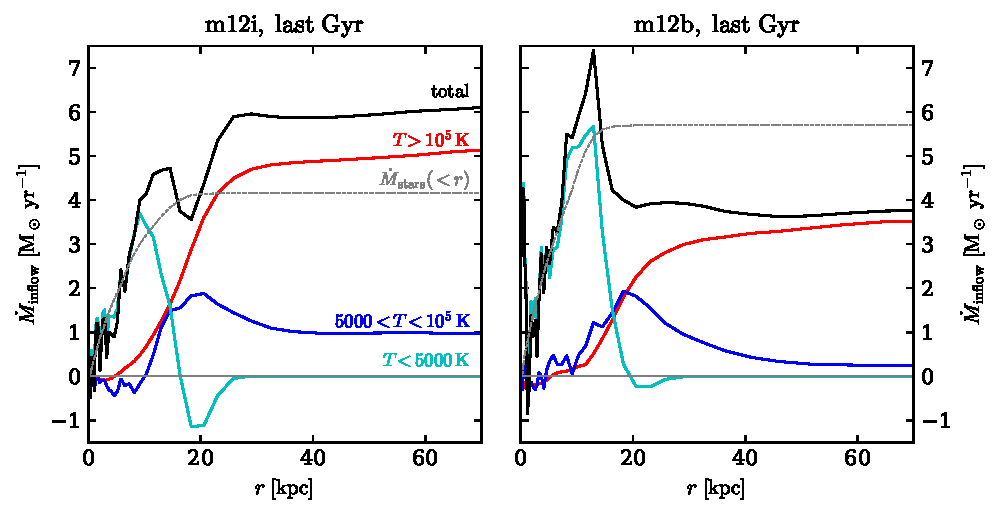
\includegraphics{Mdot.pdf}
    \caption{
    Average mass inflow rates in the last Gyr of two FIRE simulations. Black line shows the total $\dot{M}_{\rm inflows}$  while colored lines show the division into the hot, cool and cold phases. 
    The inflow is dominated by hot gas at $r\gtrsim 20 $ kpc. For comparison the dashed grey line shows the gas mass converted into stars.
    \textbf{verify conversion SFR to Mdot\_stars}
    % \textbf{Add images of face-on $z=0$ slice with temperature and velocity arrows.}
    % \textbf{Add top x-axis with radius in units of $\Rvir$}.
    % \textbf{Add cuts on density/temperature to avoid ISM gas causing a wide dispersion at low-r.}
    % \textbf{Change to linear space to emphasize halo. Cut out accretion shock.}
    % \textbf{Try using Clarke's entropy cut.}
    }
    \label{f:Mdot}
\end{figure*}

\begin{figure*}
    \centering
    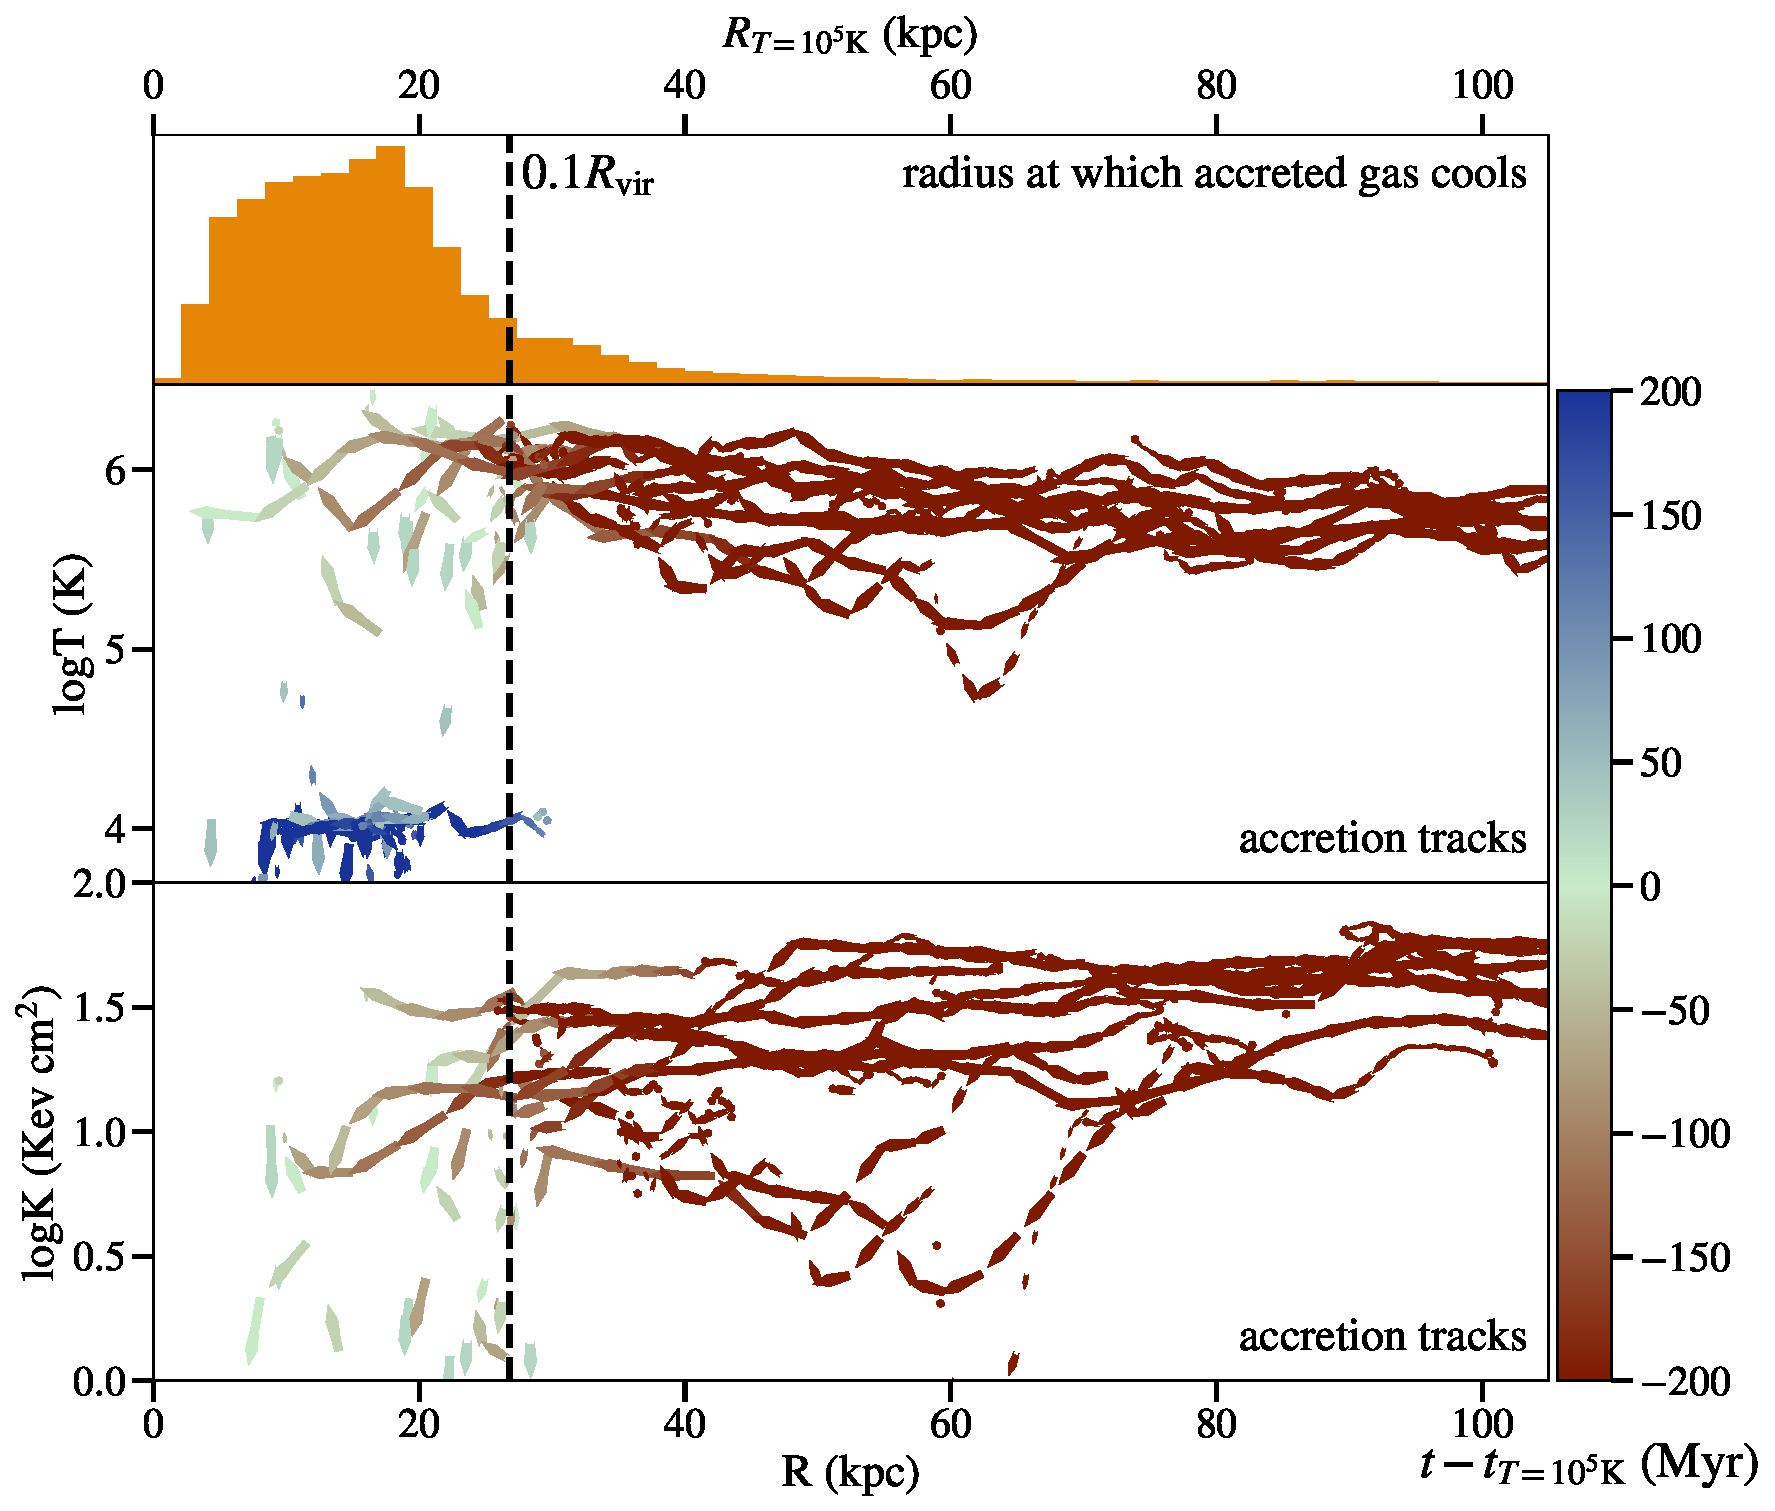
\includegraphics[width=\columnwidth]{figures/tracks_m12i_md.pdf}
    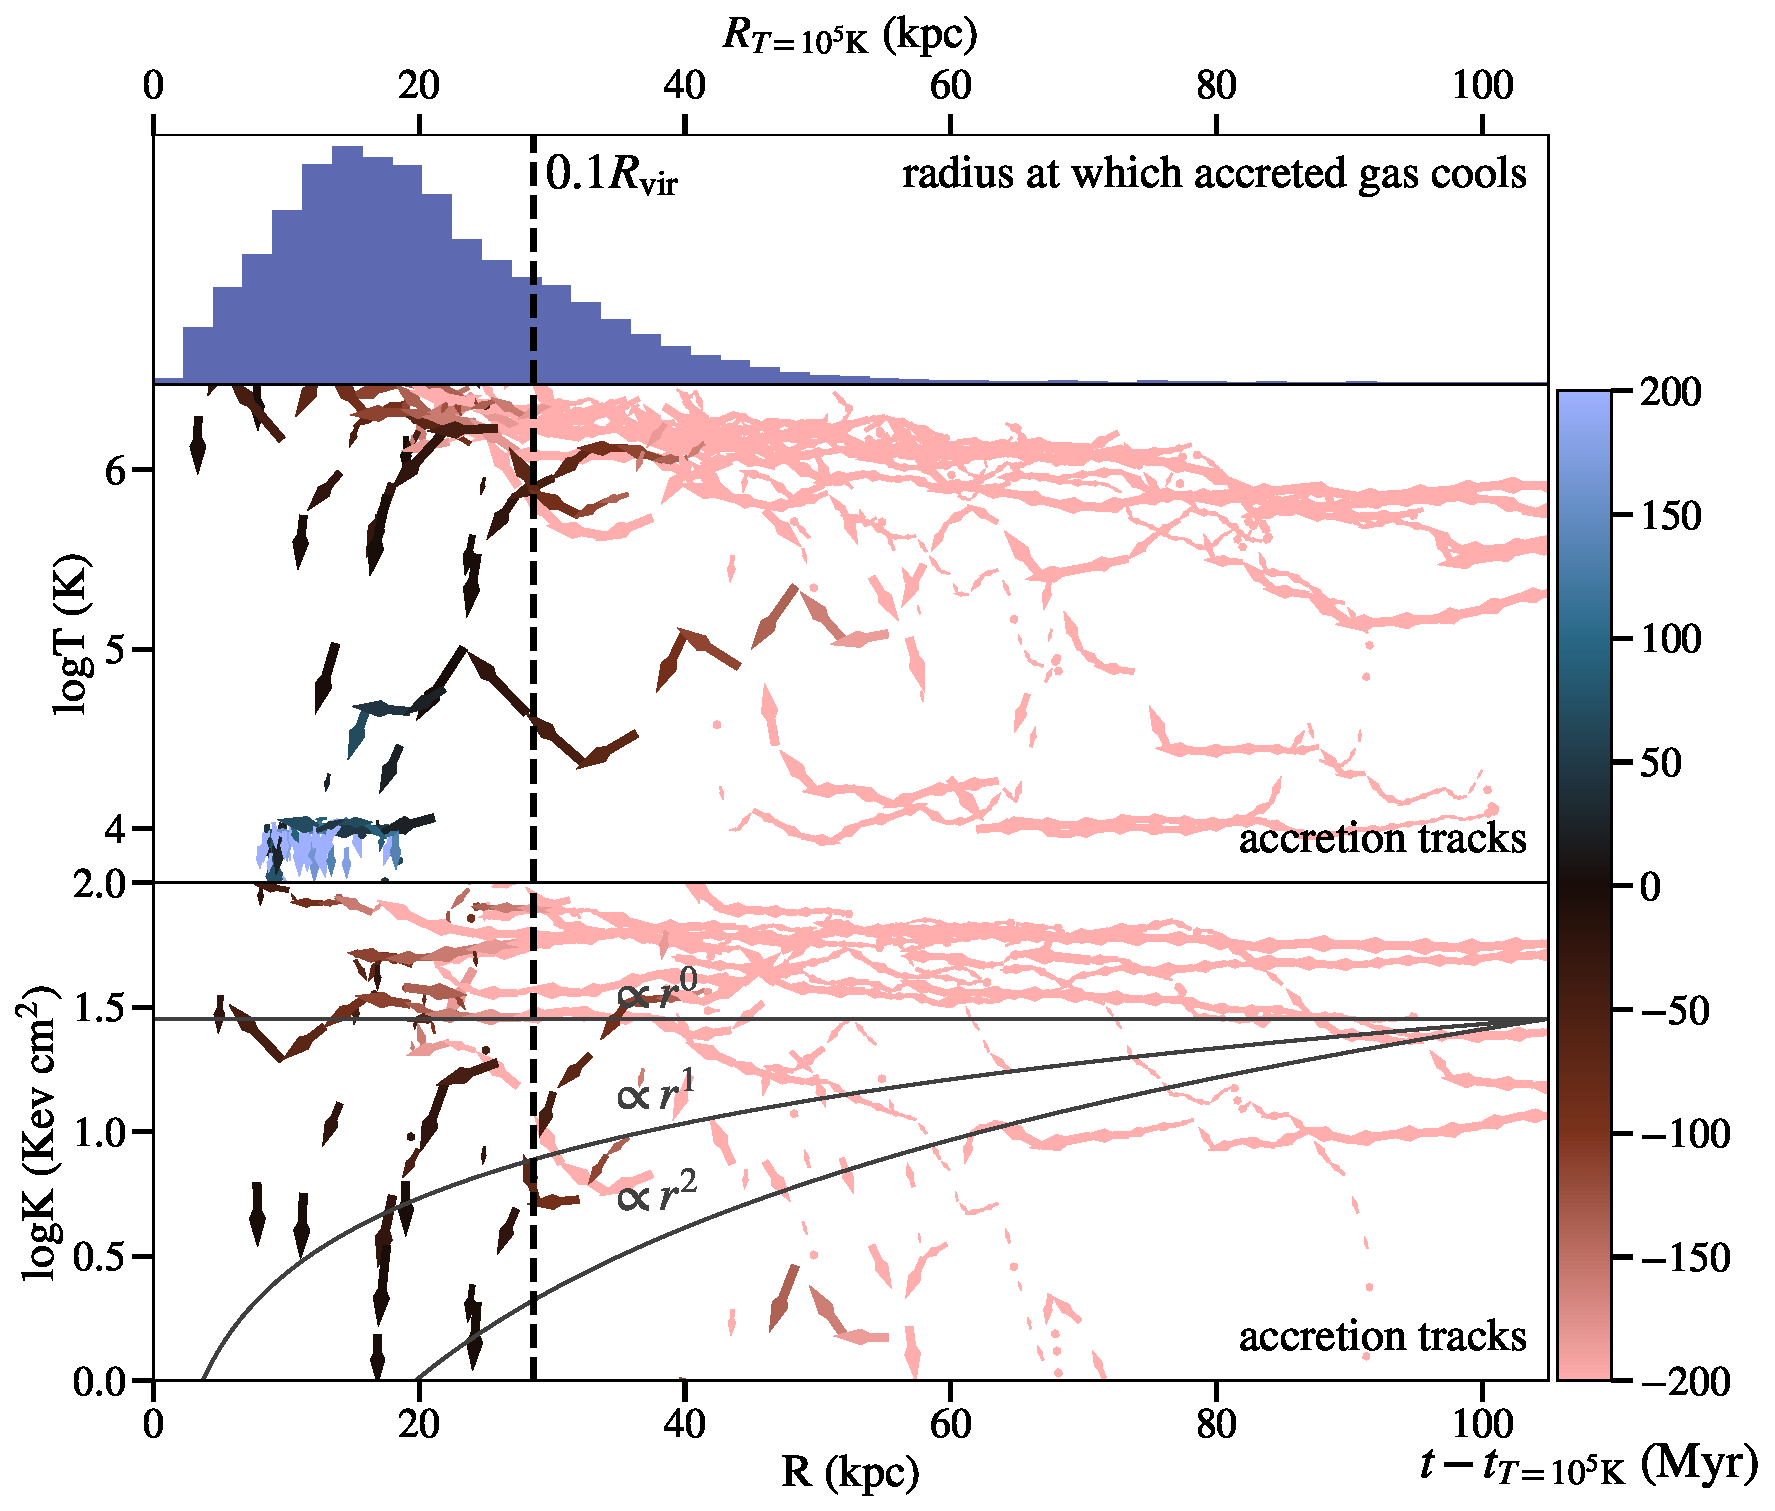
\includegraphics[width=\columnwidth]{figures/tracks_m12b_md.pdf}
    \caption{
    \textbf{Main panels:} 10 T vs.\ R and K vs.\ R tracks for two $L^\star$ halo at $z=0$, with color indicating time minus accretion time.
    Gas either remains hot or cools and reheats down to $\lesssim 0.1 R_{\rm vir}$. 
    % We do not show gas that has ever been ejected from the central galaxy.
    \textbf{Top panel:} Distribution of $\Rcool$, the radius at which gas particles last transitioned from $T > 10^5$ K to $T < 10^5$ K prior to accreting, i.e. the radius at which they cooled prior to accretion.
    \textbf{Try out fractional form: ultimate goal make it super clear (which it is, so the presentation shouldn't hinder it).}
    \textbf{Remove vertical lines for Rsonic.}
    \textbf{Consider putting histograms by themselves to have a very simple, clear result with no distraction.}
    }
    \label{f: T vs R}
\end{figure*}

% \begin{figure}
%     \centering
%     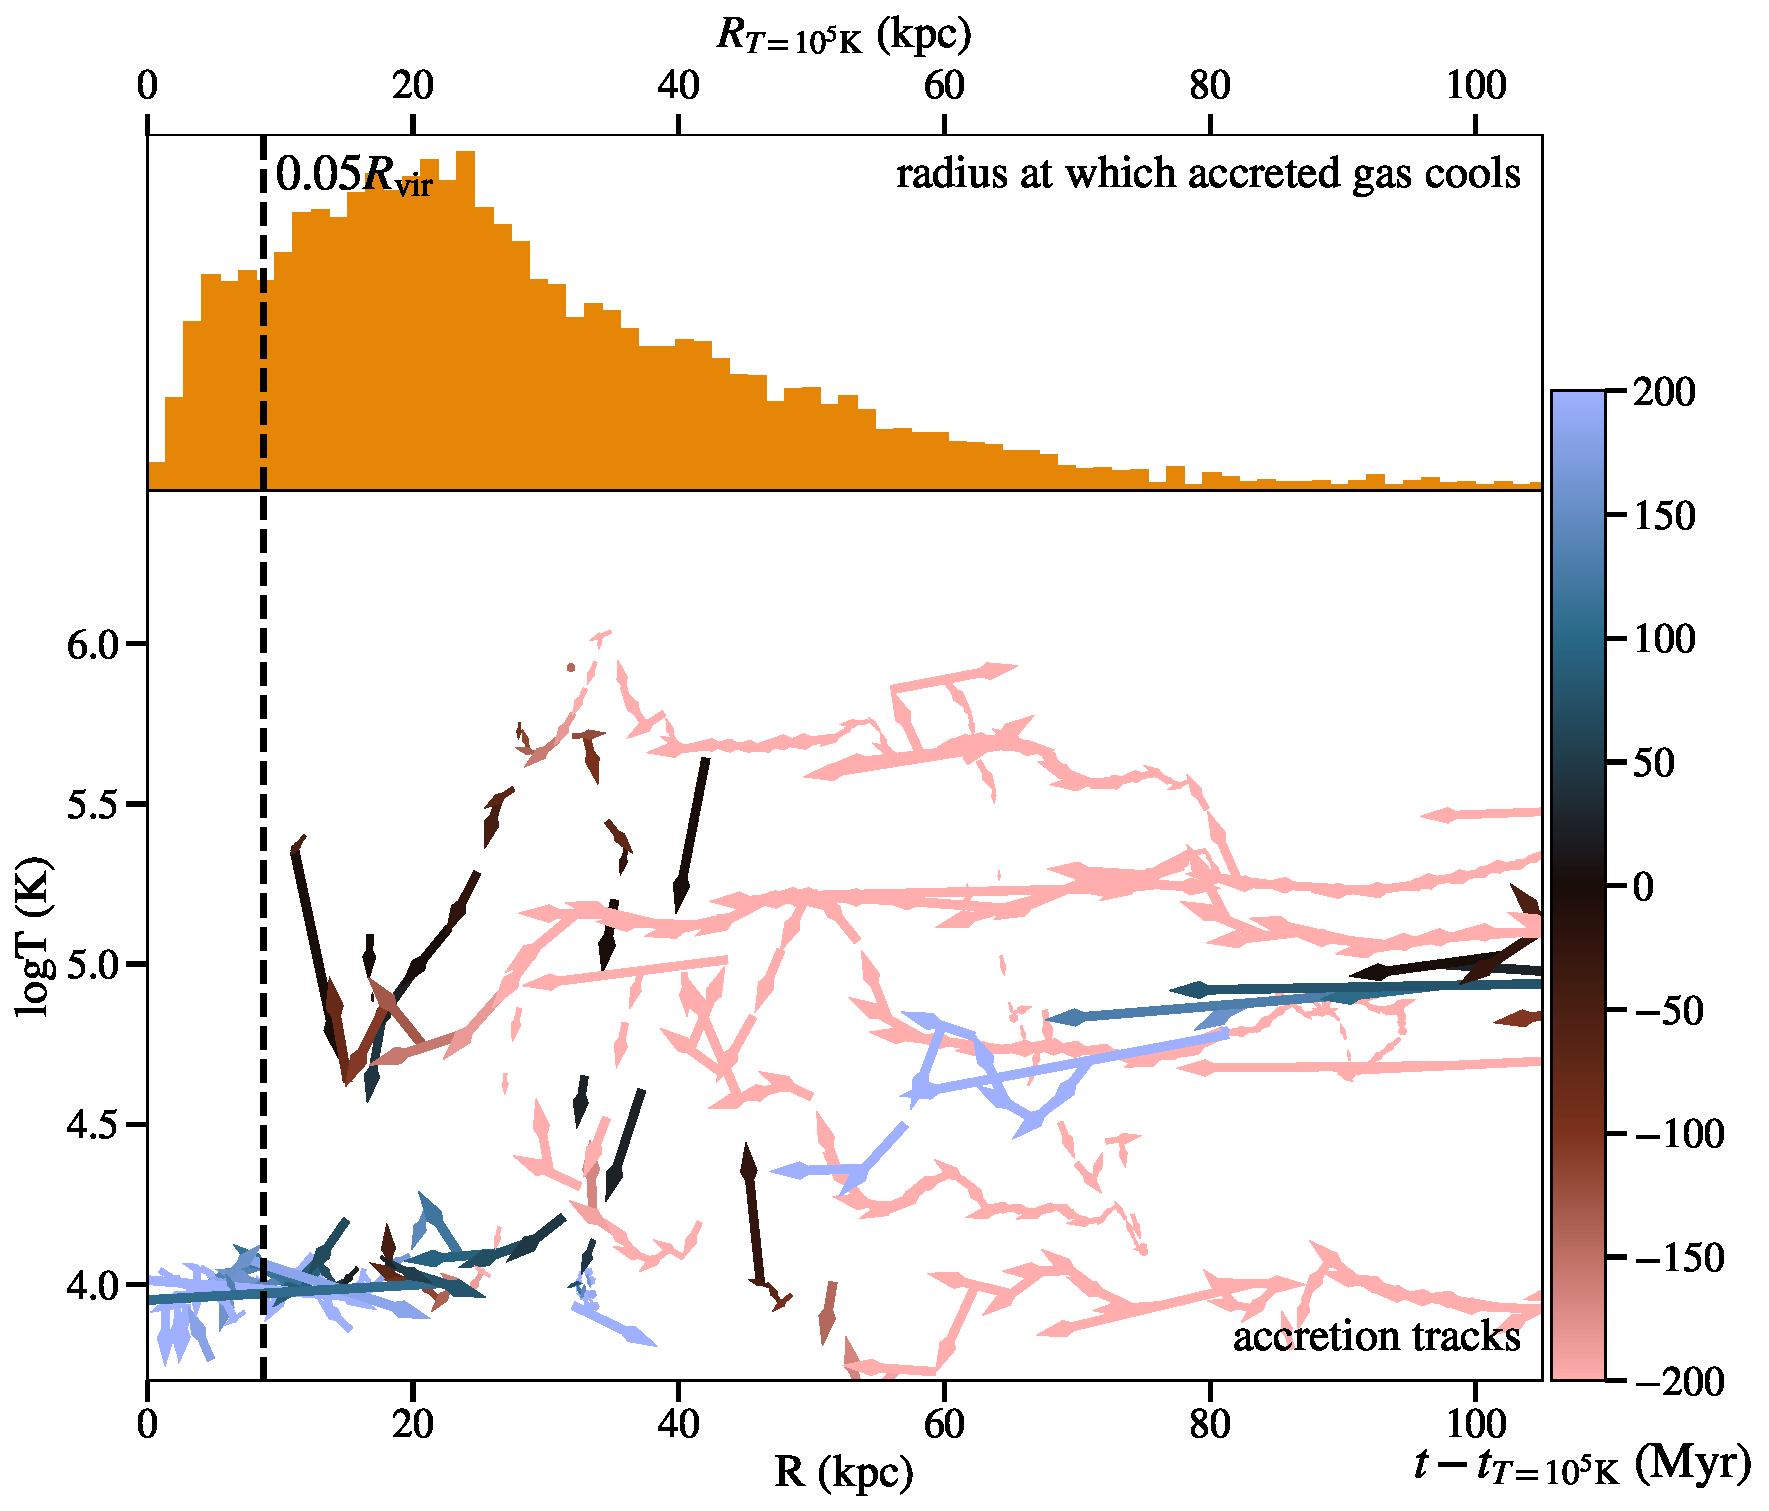
\includegraphics[width=\columnwidth]{figures/tracks_m11d_md.pdf}
%     \caption{
%     Same as Figure~\ref{f: T vs R}, but for \texttt{m11d\_md}.
%     }
%     \label{f: T vs R m11d_md}
% \end{figure}

% \begin{figure}
% \centering
% 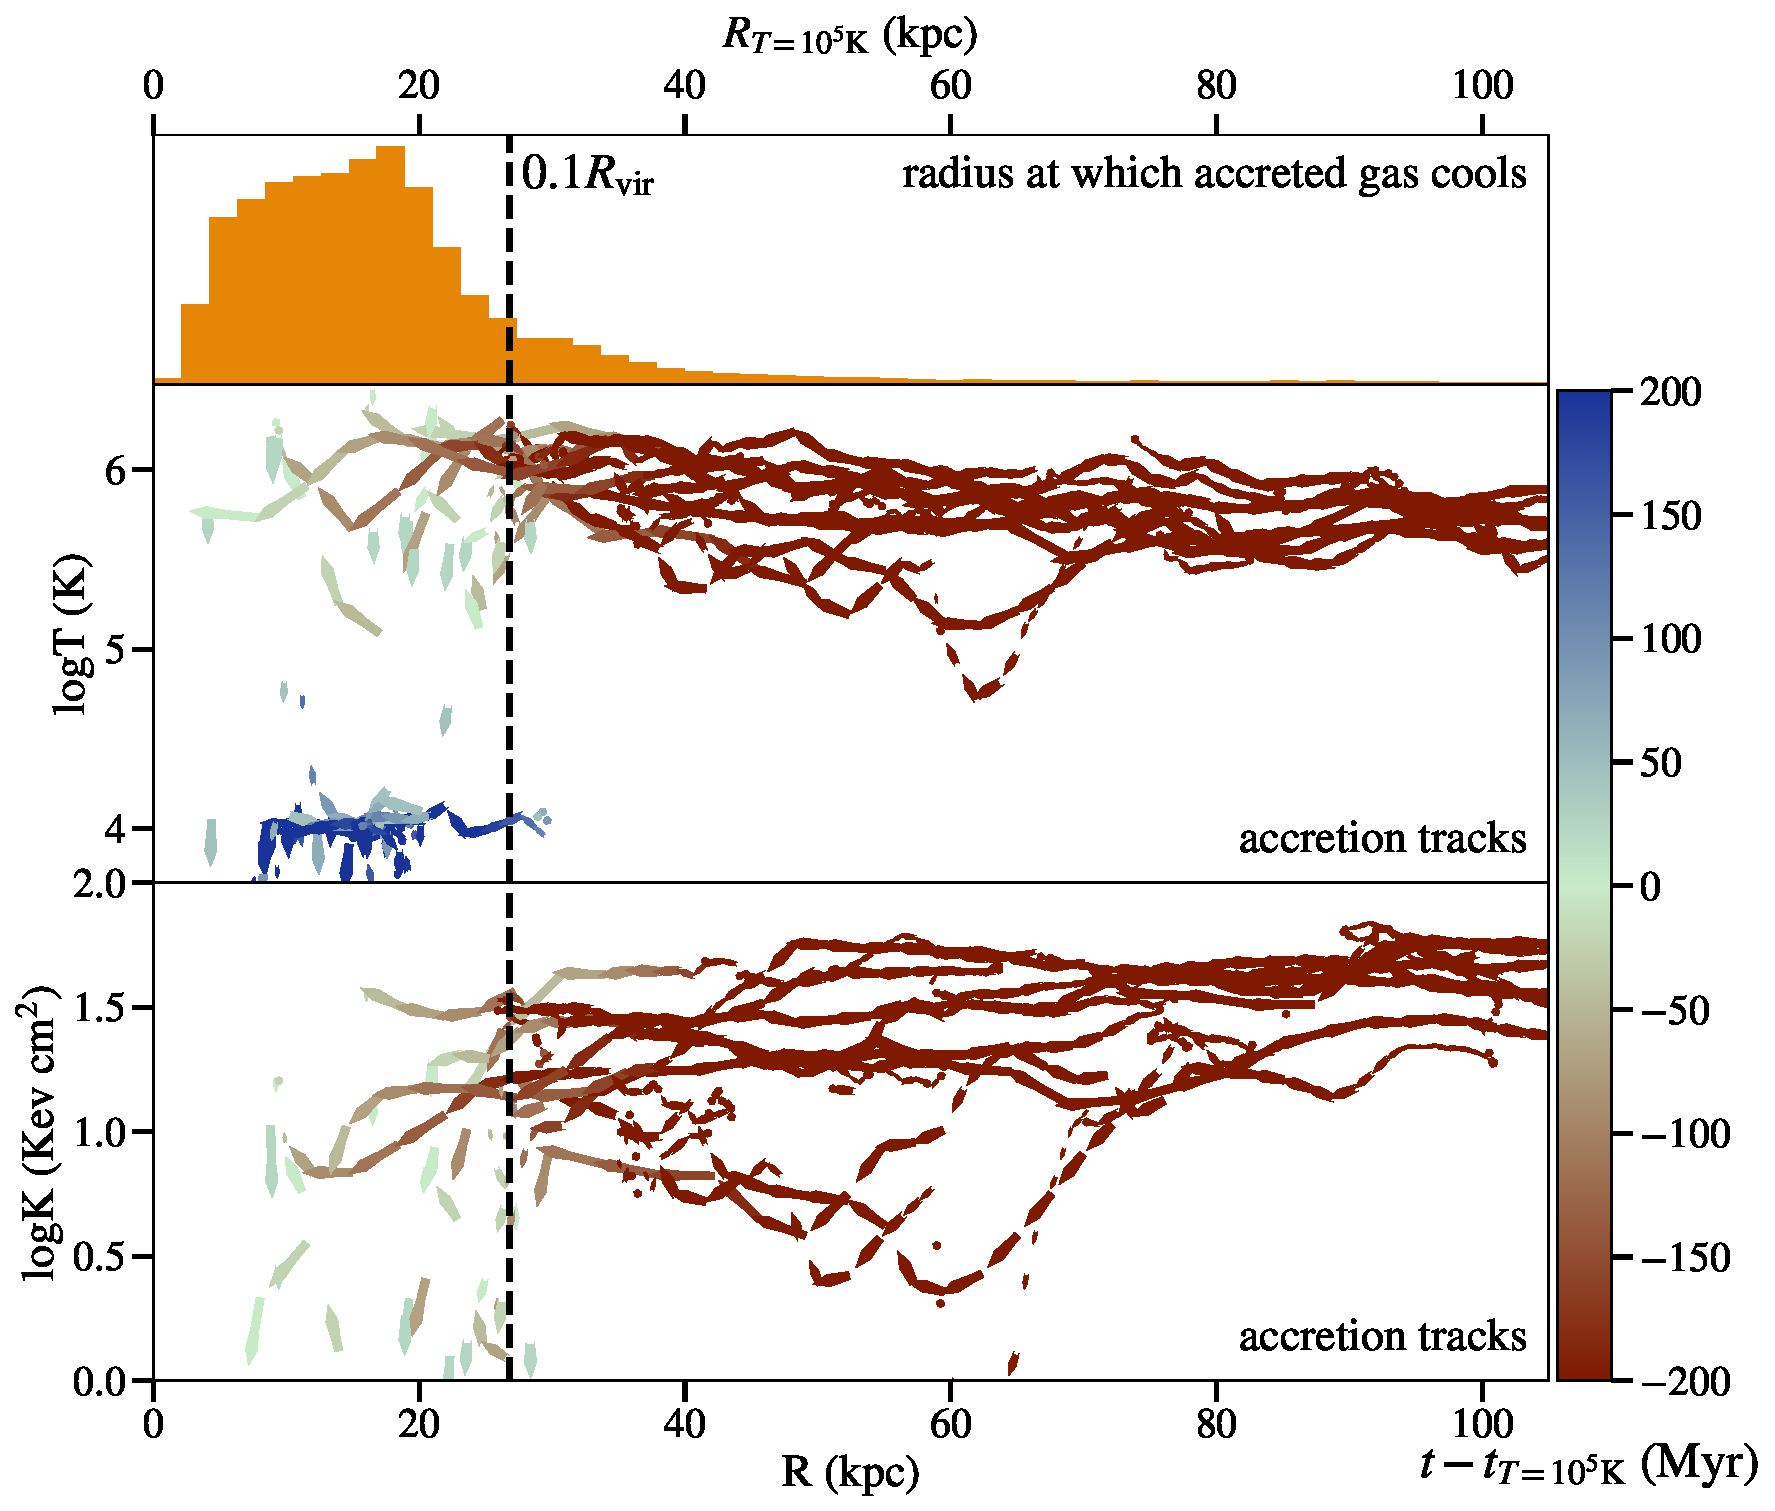
\includegraphics[width=\columnwidth]{figures/tracks_m12i_md.pdf}
% \end{figure}

\begin{figure}
    \centering
    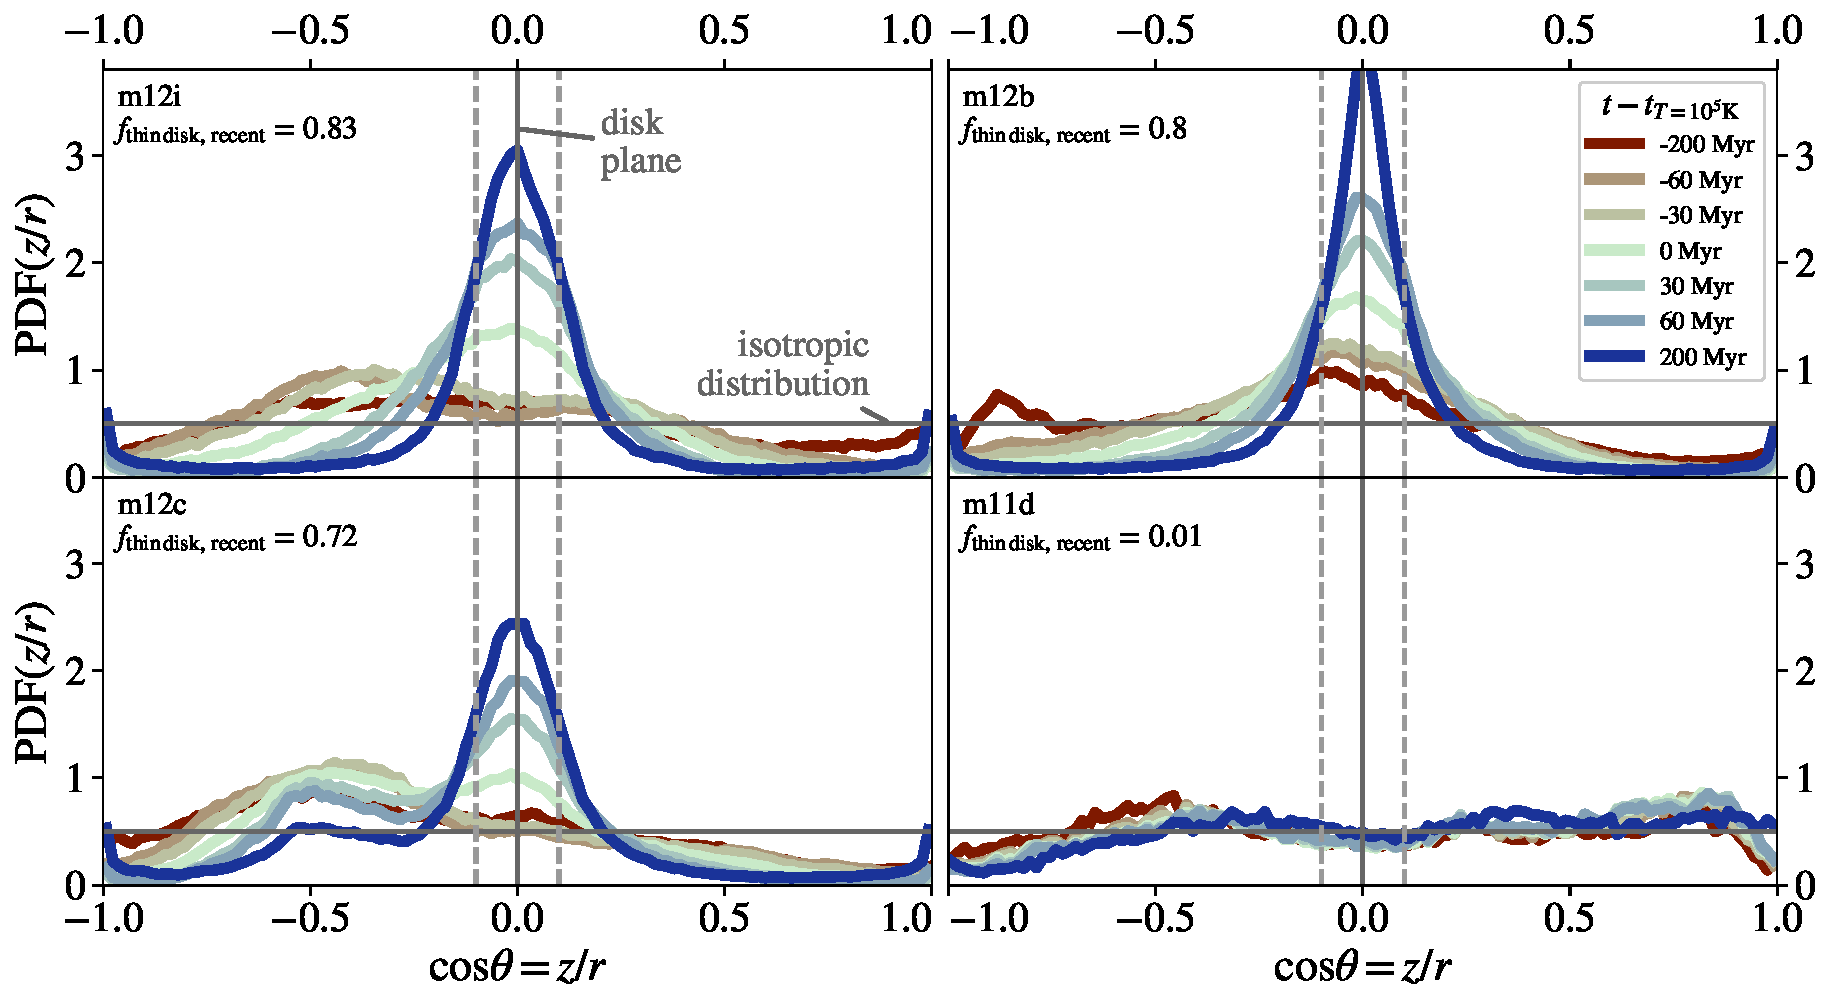
\includegraphics[width=\columnwidth]{figures/theta_vs_t.pdf}
    \caption{
    Angular distribution of accreting gas over 250 Myr before/after cooling. Cooling and circularization occur together -- prior to cooling the gas is distributed quasi-spherically, while after cooling the gas has a disc like configuration.
    \textbf{note `disc distribution' near vertical line'}.
    \textbf{remove m11d maybe. An advantage for including is that it provides a powerful contrast.}.
    \textbf{Try splitting up into two panels side-by-side with a "before" panel and an "after" panel.}
    \textbf{Make a plot using the same particle bins as here, but showing the sum of the angular momentum for all particles in the bin, divided by vcR}
    \textbf{See if the distribution becomes narrower if selecting a narrower range of particles.}
    \textbf{Compare accretion radii (this plot) to a textbook angular momentum support radii distribution.}
    }
    \label{f: theta vs R}
\end{figure}

\begin{figure}
% 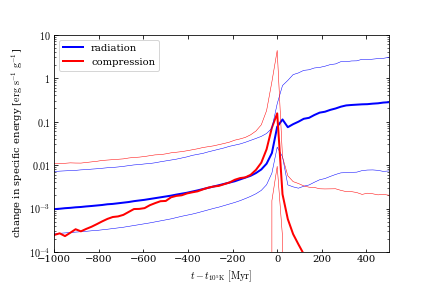
\includegraphics[width=\columnwidth]{rad_vs_compress.png}
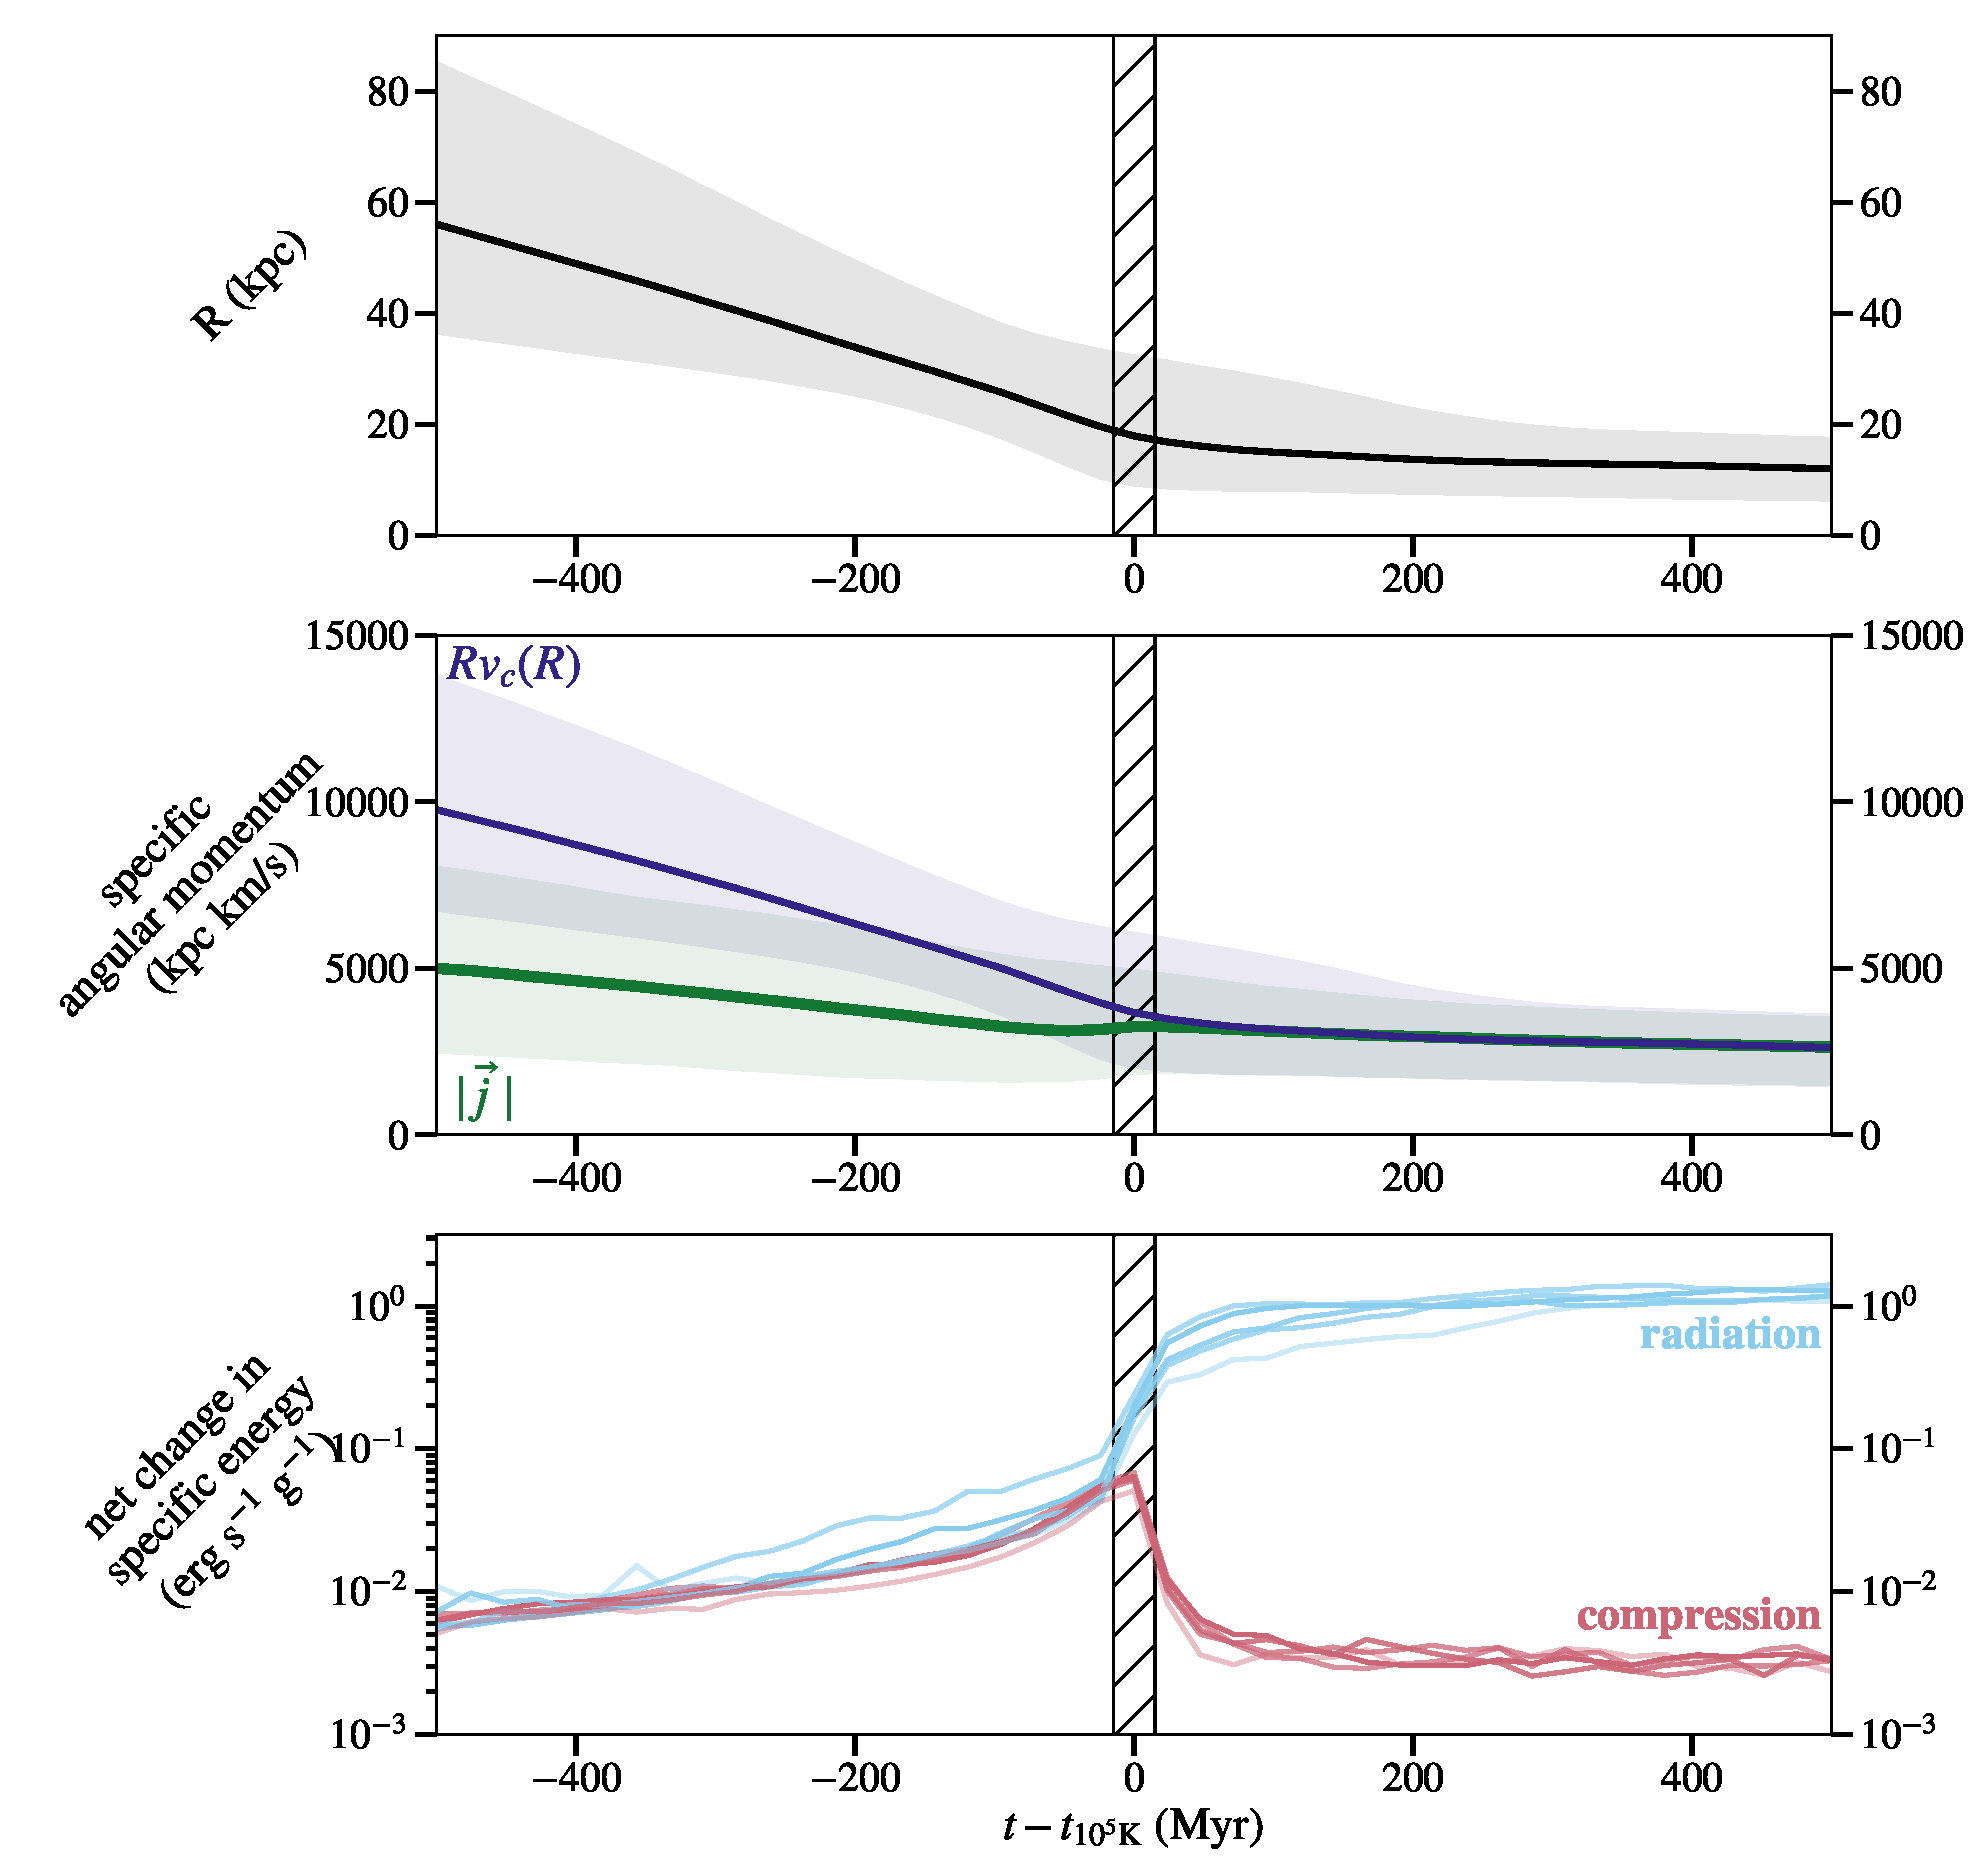
\includegraphics[width=\columnwidth]{figures/rad_vs_compress.pdf}
% 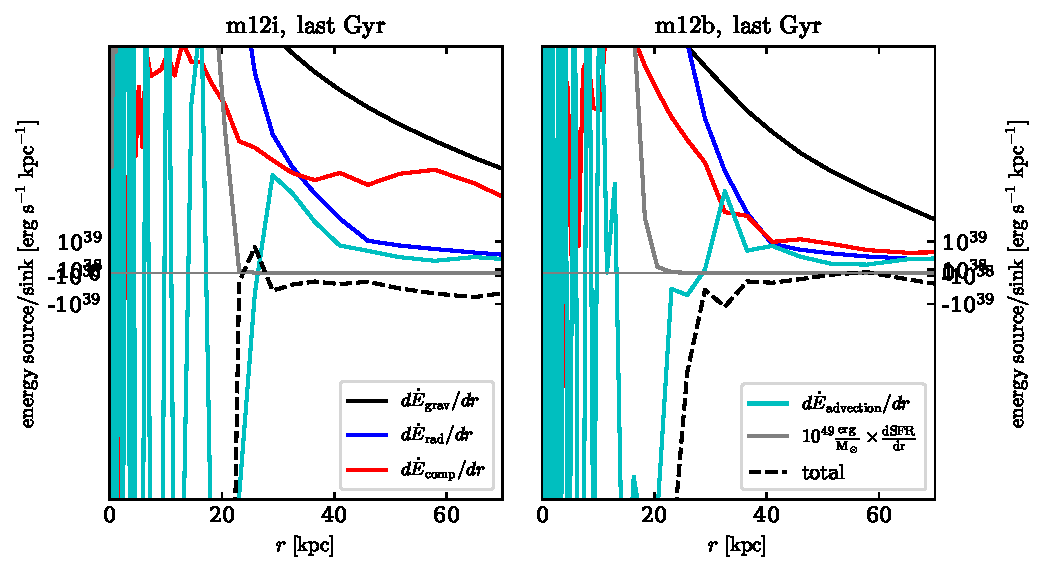
\includegraphics{Edot.pdf}
\caption{
% Comparison of energy sources and sinks in the last Gyr of two FIRE simulations. Black line shows the gravitational energy loss of the flow.  Blue line shows the energy lost to radiation of $T>10^4$ K gas. Red line shows the $PdV$ work on the flow. Gray dashed lines approximate the feedback energy. 
This figure shows that gas cools when the cooling is no longer offset by compressive heating.
\textbf{
Add another panel that shows average radius for the same collection of particles.
Try cutting out tail of particles that makes the low-opacity lines.
Radiation -> radiation cooling
Compression -> compression heating
Add "time" to the x-axis.
}
}
\label{f:Edot}
\end{figure}

\begin{figure}
    \centering
    % \includegraphics{}
    \caption{
    \textbf{
    Left:
    Stellar profile for young edge-on stellar disk showing truncation.
    Include vertical line for Rcirc (top panels for Figure 2-3).
    Right:
    Observational histogram for Rtrunc/Rhalf, with a line for the FIRE sim value.
    }
    }
    \label{f:emission}
\end{figure}

\begin{figure}
    \centering
    % \includegraphics{}
    \caption{
    \textbf{Spare figure, but maybe
    cooling emission in X-ray, optical and UV lines vs.\ radius, only from tracked particles
    }
    }
    \label{f:emission}
\end{figure}

% Accretion tracks figure description
\textit{
The main panels of Figure~\ref{f: T vs R} show the paths in temperature-radius and entropy-radius space taken by accreting particles.
}

% Distribution of r1e5
\textit{
As an explicit example of how far our distribution is from a condensation model, isotropic cooling occurring randomly within $R_{\rm vir}$ would cool in a wide distribution with a median at $0.8 R_{\rm vir}$, while for our accreted gas the median $\Rcool \approx 0.06 R_{\rm vir}$.
}
\textit{We added all particles with $\Rcool>100$ to $R=100$ bin, so we don't ignore them.}

\subsection{Energetics}

To demonstrate that the hot radial inflow is driven by cooling, we compare the different terms of the energy conservation equation. In steady-state, and assuming the gravitationaly potential is constant,  energy conservation in the radial direction dictates \citep[e.g.][]{Shu82}
\begin{equation}\label{e:energy}
    \rho g v_r + H_{\rm feedback} - \frac{d}{dr}(v_r P)= 
    \frac{d}{dr}\left(\rho v_r \left(\epsilon+\frac{1}{2}v^2\right)\right)  +  \nH^2\Lambda  
\end{equation}
where the terms on the left hand side are the `source terms' -- gravity, feedback, and the work done on the shell by adjacent shells, while the terms on the right represent respectively the heating and acceleration of the flow and radiative losses. 
Integrating over radial shells and rearranging we get the energy integral
\begin{equation}
    \Mdot\frac{d}{dr}\left(\Phi+\frac{3}{2}\epsilon + \frac{1}{2}v^2\right) = 4\pi r^2 \left(\langle\nH^2\Lambda\rangle-\langle H_{\rm feedback}\rangle\right)
\end{equation}

In Fig.~\ref{f:Edot} we plot each of the terms in eqn.~(\ref{e:energy}), averaged over radial shells and over time. Shell averages of quantity $Q$ are calculated via 
\begin{equation}
    \frac{d\dot{E}_Q}{d r} = \frac{\int_{\rm shell} Q\rho^{-1} dm}{\Delta r} 
\end{equation}
where the intergral is over all particles within the shell and $\Delta r$ is the thickness of the shell. The factor $\rho^{-1}$ is since eqn.~\ref{e:energy} is in Eulerian form. We then take the average of all shells at a given $r$ in snapshots of the last Gyr of the simulation. 
% In order to calculate the compression term from a single snapshot, we make the following further approximation \textbf{(TBD: check if justified)}
% \begin{equation}
%     \frac{d\dot{E}_{\rm comp}}{d r} \approx 
%     \Mdot P \left\langle\frac{d V}{d r}\right\rangle_{\rho v_r} \approx
%     \Mdot P \frac{d\langle V \rangle_{\rho v_r} }{dr}
% \end{equation}
% Note that since $d\ln\rho/ d\ln r$ is of order unity, and in hot virial temperature gas $\epsilon/r \approx c_{\rm s}^2/r \approx v_{\rm c}^2/r = g$, we get that $\dot{E}_{\rm comp}$ (eqn.~\ref{e:Ecomp}) and $\dot{E}_{\rm grav}$ (eqn.~\ref{e:Egrav}) are of the same order.
\section{Discussion}


\subsection{AGN feedback}

\textit{
\begin{itemize}
    \item Results expected to be valid after disc forms (Paper III) and before AGN feedback kicks in (ref.~Byrne+)
    \item Results are baseline for detecting effects of feedback in observations / simulations
\end{itemize}
}

\subsection{Contrast with other accretion mechanisms}

\subsubsection{Condensation/Precipitation}

\begin{itemize}
    \item Nelson+20
    \item Esmerian+20
\end{itemize}
emphasize cold clouds due to over-densities heat back up and join the hot inflow, as in Illustris (see fig.~12 in Nelson+20

\subsubsection{filaments}
Kretschmer+20

\textbf{Discuss resolution effects and Balbus\&Soker}

\section{Conclusions}

\textbf{TBD.}

\section*{Acknowledgements}

\textbf{TBD.}


%%%%%%%%%%%%%%%%%%%%%%%%%%%%%%%%%%%%%%%%%%%%%%%%%%

%%%%%%%%%%%%%%%%%%%% REFERENCES %%%%%%%%%%%%%%%%%%

% The best way to enter references is to use BibTeX:

\bibliographystyle{mnras}
\bibliography{example} % if your bibtex file is called example.bib

% Alternatively you could enter them by hand, like this:
% This method is tedious and prone to error if you have lots of references
%\begin{thebibliography}{99}
%\bibitem[\protect\citeauthoryear{Author}{2012}]{Author2012}
%Author A.~N., 2013, Journal of Improbable Astronomy, 1, 1
%\bibitem[\protect\citeauthoryear{Others}{2013}]{Others2013}
%Others S., 2012, Journal of Interesting Stuff, 17, 198
%\end{thebibliography}

%%%%%%%%%%%%%%%%%%%%%%%%%%%%%%%%%%%%%%%%%%%%%%%%%%

%%%%%%%%%%%%%%%%% APPENDICES %%%%%%%%%%%%%%%%%%%%%

\appendix

\section{Angular Momentum of Accreting Material}

% \begin{figure}
%     \centering
%     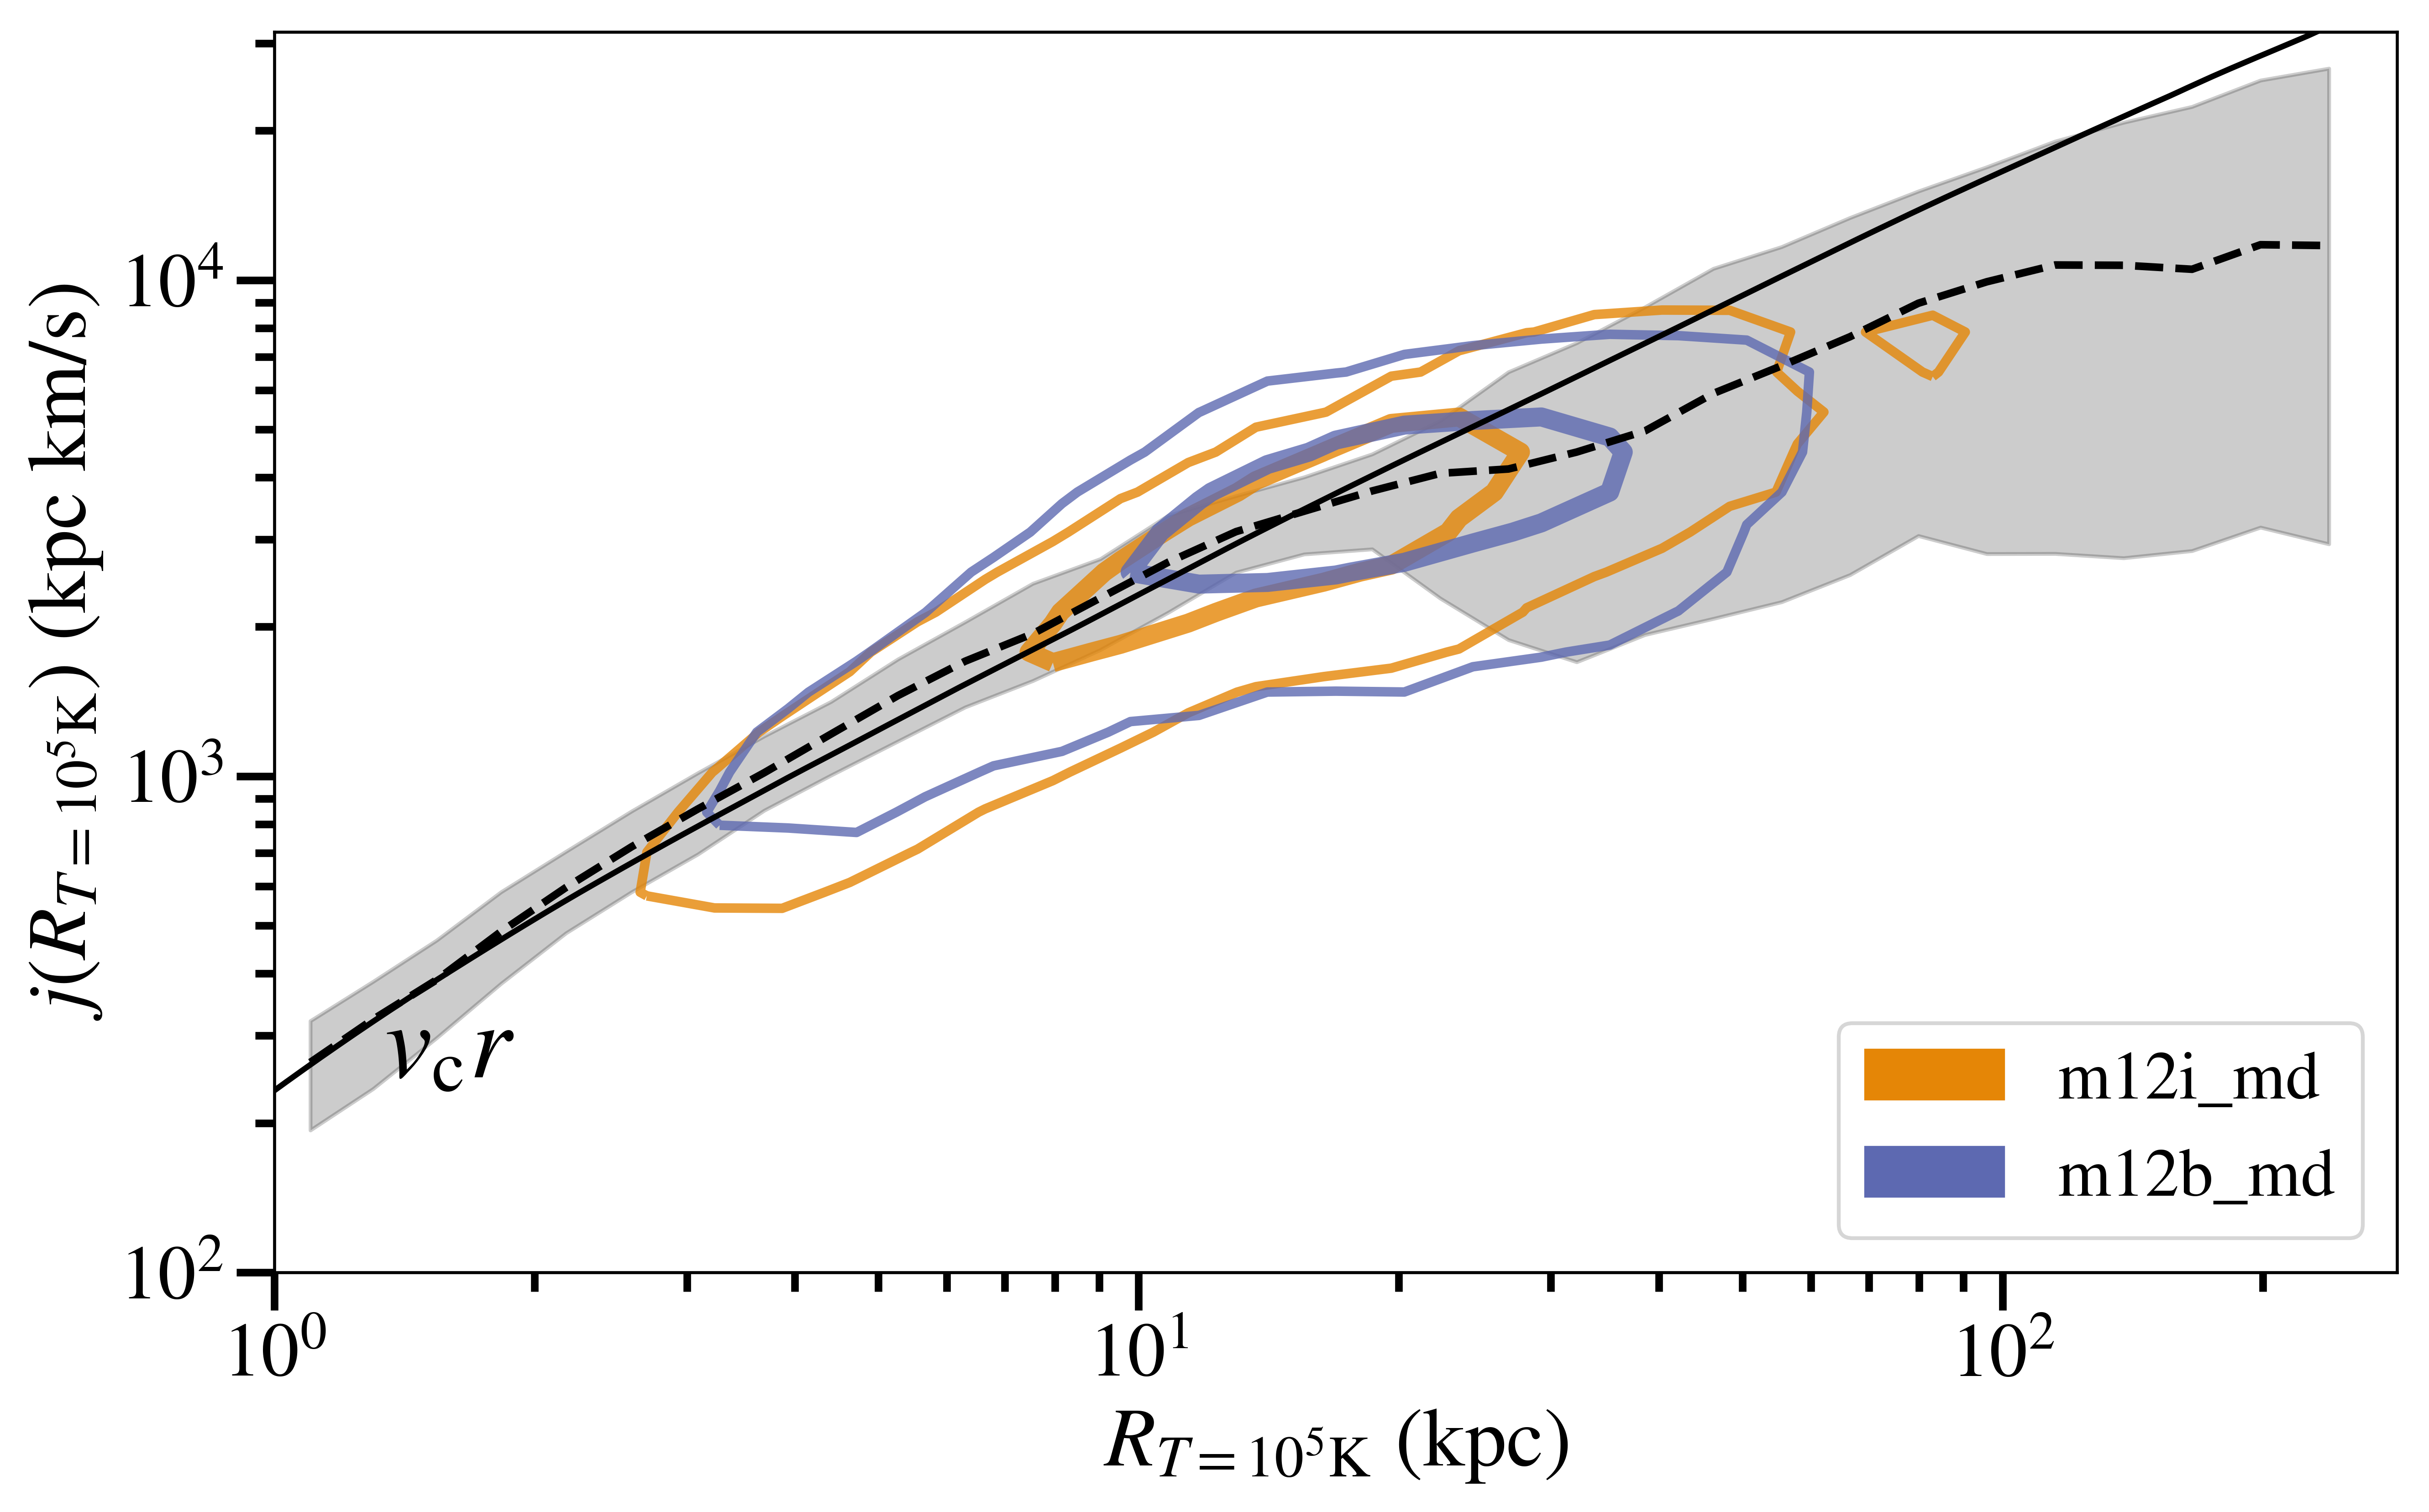
\includegraphics[width=\columnwidth]{figures/j_vs_rcondense.png}
%     \caption{
%     Distribution of $\Rcool$ vs j($\Rcool$) for four FIRE-2 halos with $L(z=0) \sim L^\star$.
% Thick (thin) contours enclose values for 50\% (90\%) of the accreted gas particles.
% The angular momentum as a function of radius for all gas in \texttt{m12i} at $z=0$ is displayed as a dashed line (the median) and shaded regions (5th-95th percentiles).
% \textbf{
% Maybe delete this figure later, because it's only relevant for simulations that have a wide distribution of $\Rcool$, which are only the artificially wide non-md runs.
% }
% \textbf{Is the 100 kpc-cooling gas related to satellite galaxies?}
% \textbf{Try changing shaded region to only hot gas instead of all gas.}
% \textbf{Try histogram of r/(j/vc) instead, to demonstrate that that decreases the spread.}
% \textit{
% In all halos the distributions are consistent with $j_{\rm c} = v_{\rm c} r$, i.e. gas cools once circularized.
% This demonstrates that the variable angular momentum of incoming gas drives the width in the $\Rcool$ distribution.
% }
%     }
%     \label{f: jcool vs Rcool}
% \end{figure}

\section{Metal diffusion vs non-metal diffusion vs MHDCV}

\textbf{Plot of distribution $\Rcool$ for m12i and m12i\_md overlapping. Show cooling only happens at large radii in metal diffusion sims.}

\textbf{Add mhdcv comparison.}

%%%%%%%%%%%%%%%%%%%%%%%%%%%%%%%%%%%%%%%%%%%%%%%%%%


% Don't change these lines
\bsp	% typesetting comment
\label{lastpage}
\end{document}

% End of mnras_template.tex
